\section*{Problema 01}

\textbf{Explora en
	\url{https://colab.research.google.com/drive/1pwCqLdvxeqChzDG3MoFIgR7m6lsInKs5?usp=sharing} el efecto de cambiar los parámetros en una SVM y convéncete que es de acuerdo a (congruente con) el funcional de costo de una SVM.}

\subsection*{Experimento 1}

\textbf{¿Cuál es el efecto de cambiar el parámetro $\lambda$/$\gamma$ (cost)?}

\begin{figure}[H]
	\centering
	\begin{subfigure}{4cm}
		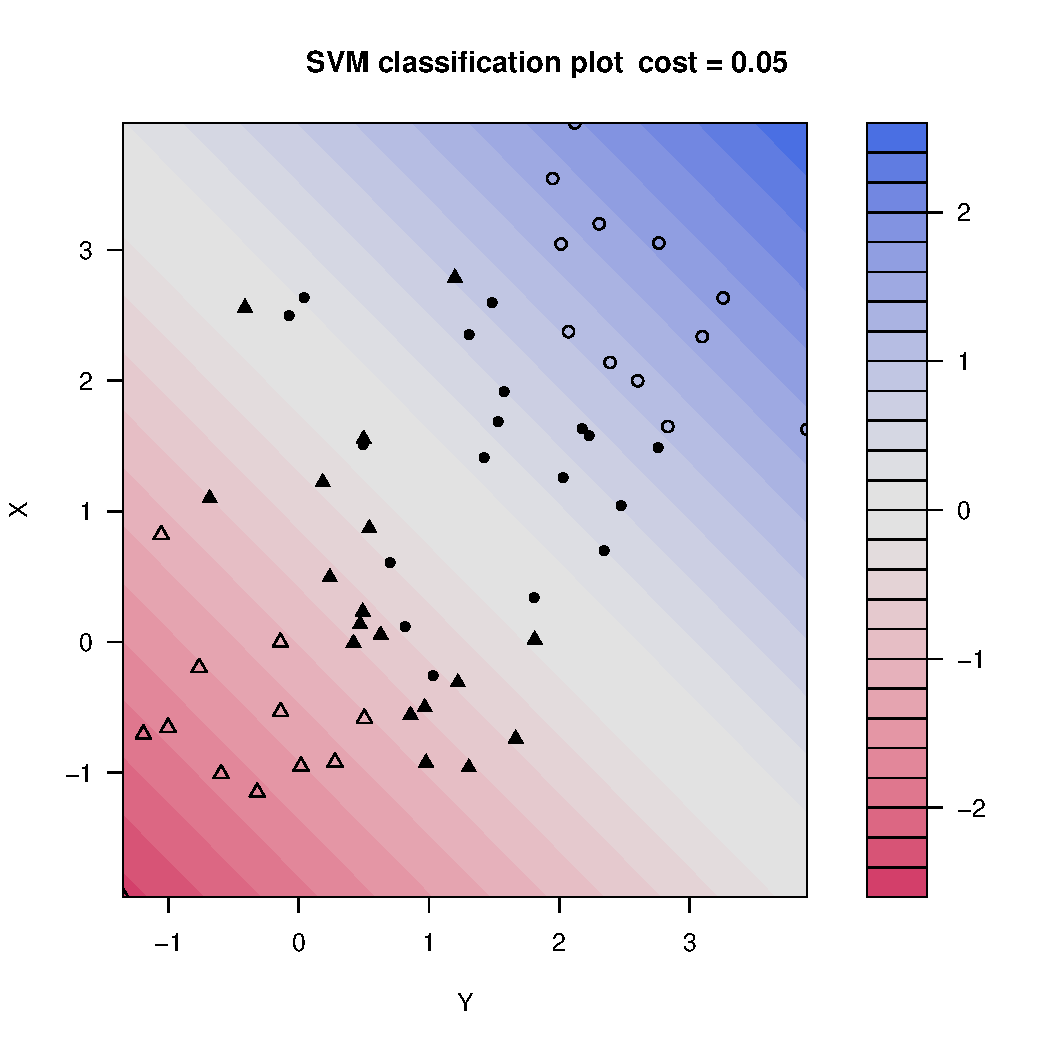
\includegraphics[width=4cm]{Graphics/Problema_01/Experiment_01_1.pdf}
		\caption{}
	\end{subfigure}
	\begin{subfigure}{4cm}
		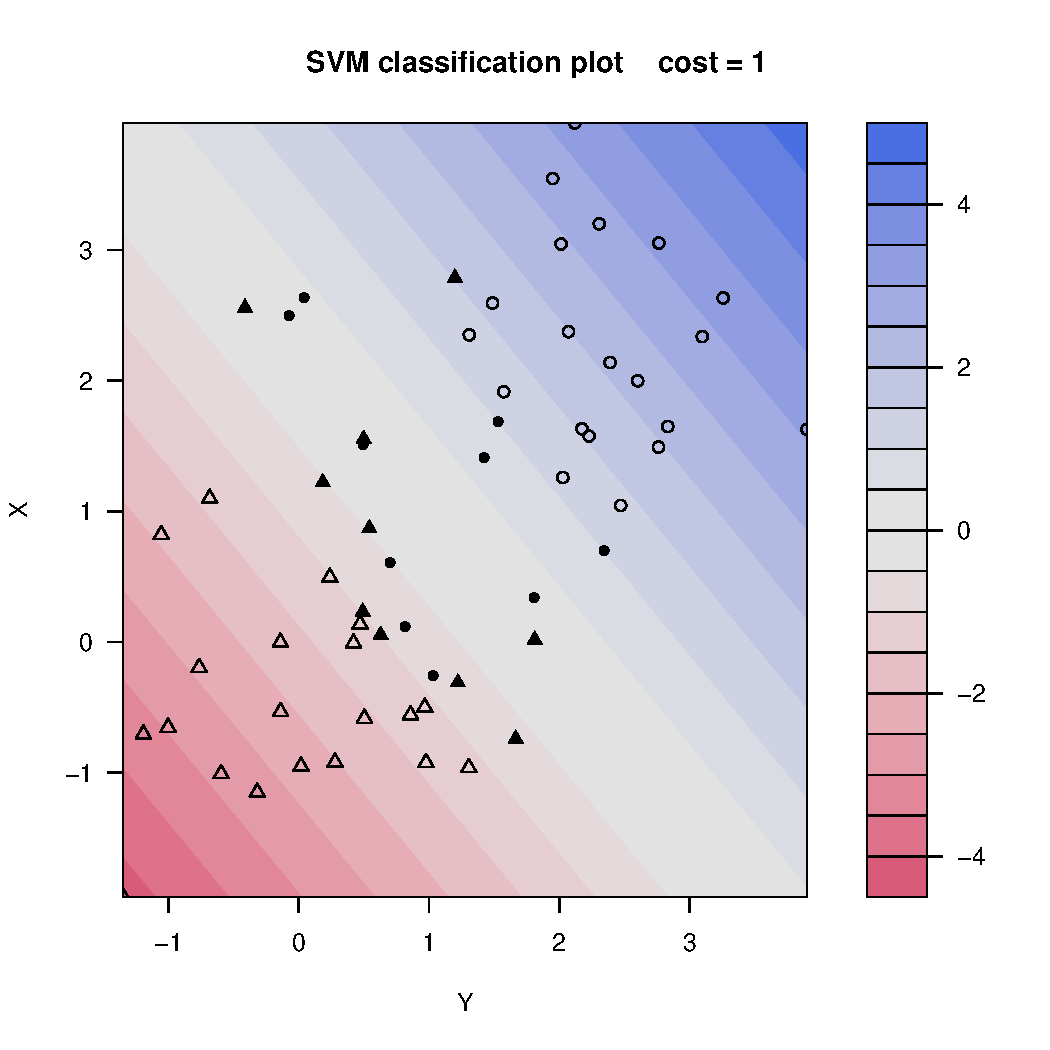
\includegraphics[width=4cm]{Graphics/Problema_01/Experiment_01_2.pdf}
		\caption{}
	\end{subfigure}
	\begin{subfigure}{4cm}
		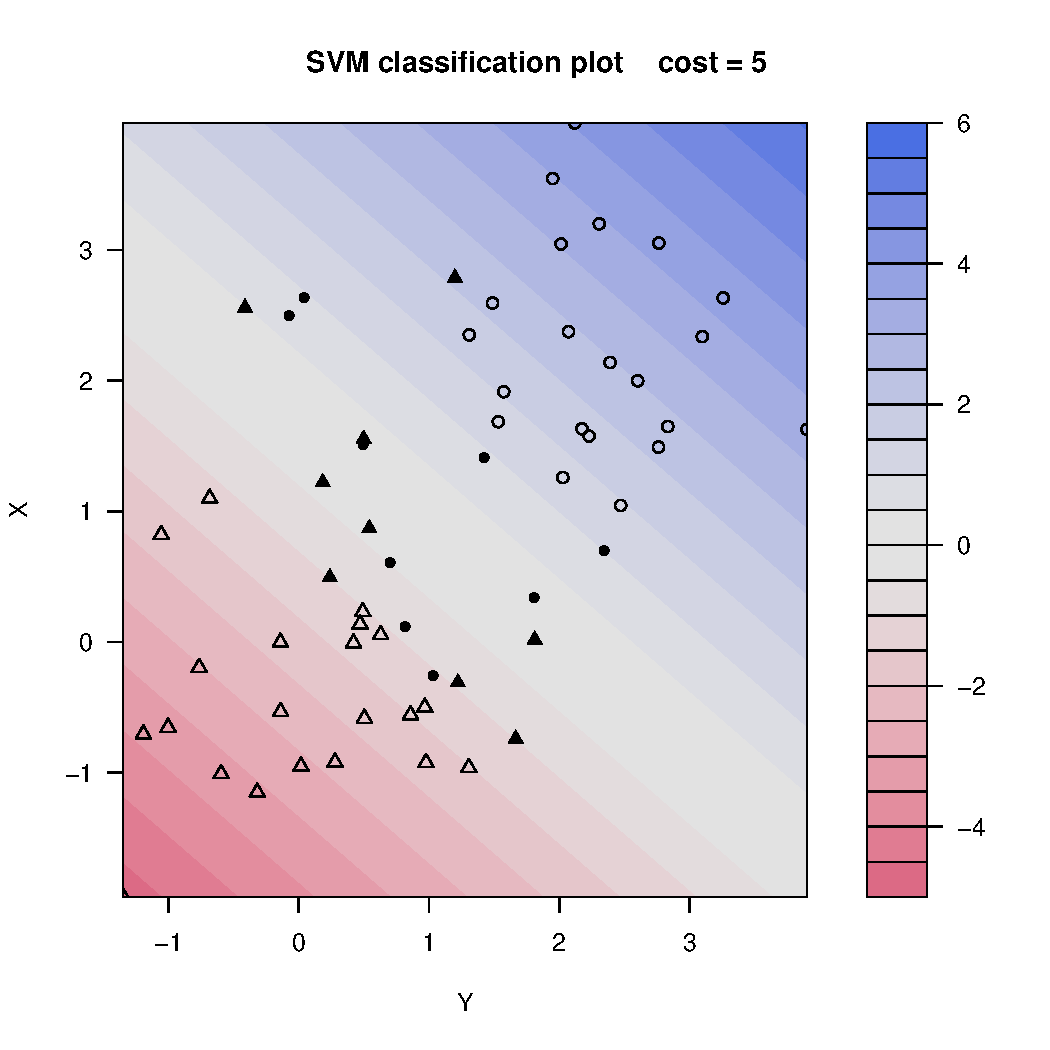
\includegraphics[width=4cm]{Graphics/Problema_01/Experiment_01_3.pdf}
		\caption{}
	\end{subfigure}
	\begin{subfigure}{4cm}
		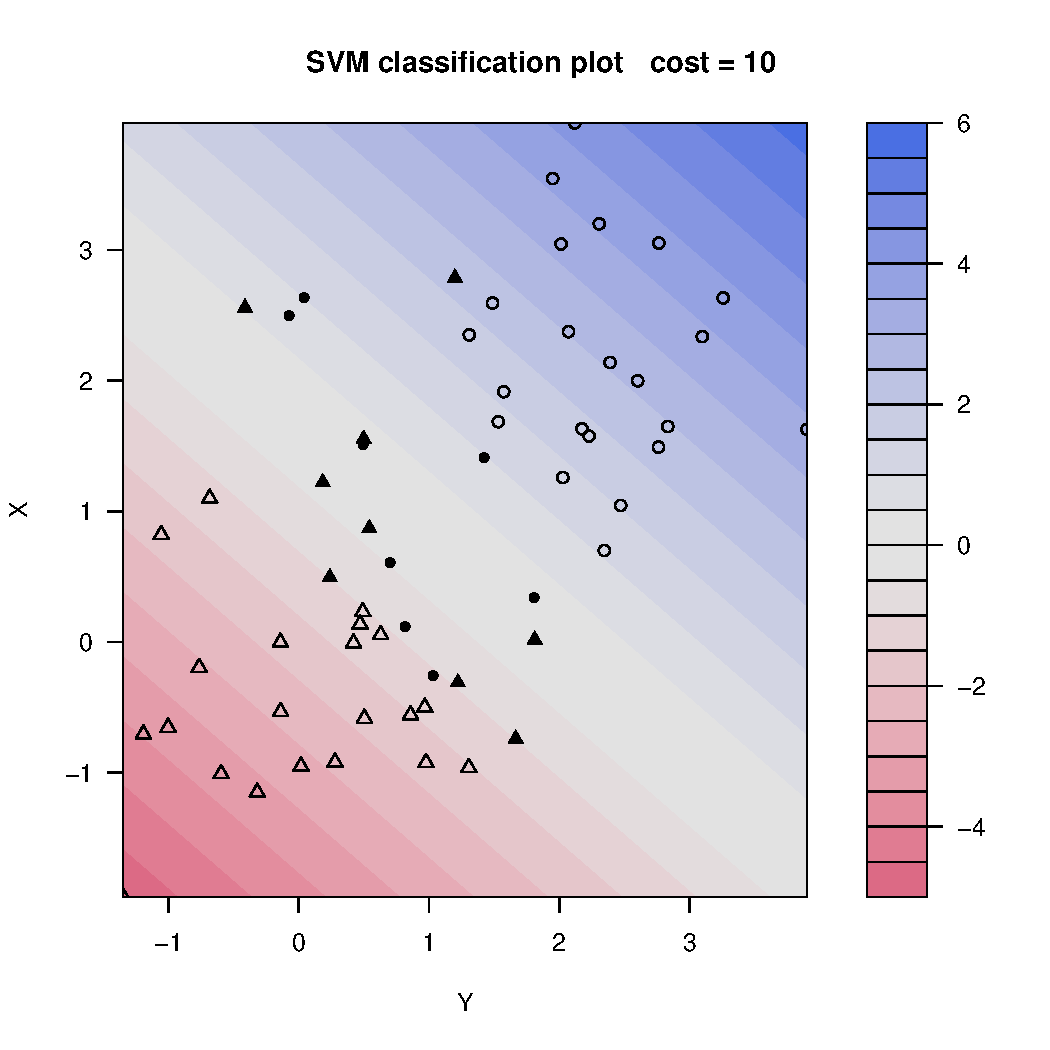
\includegraphics[width=4cm]{Graphics/Problema_01/Experiment_01_4.pdf}
		\caption{}
	\end{subfigure}
	\caption{}
\end{figure}

\subsection*{Experimento 2}

\textbf{¿Cuál es el efecto de aumentar el grado de polinomio?}

\begin{figure}[H]
	\centering
	\begin{subfigure}{4cm}
		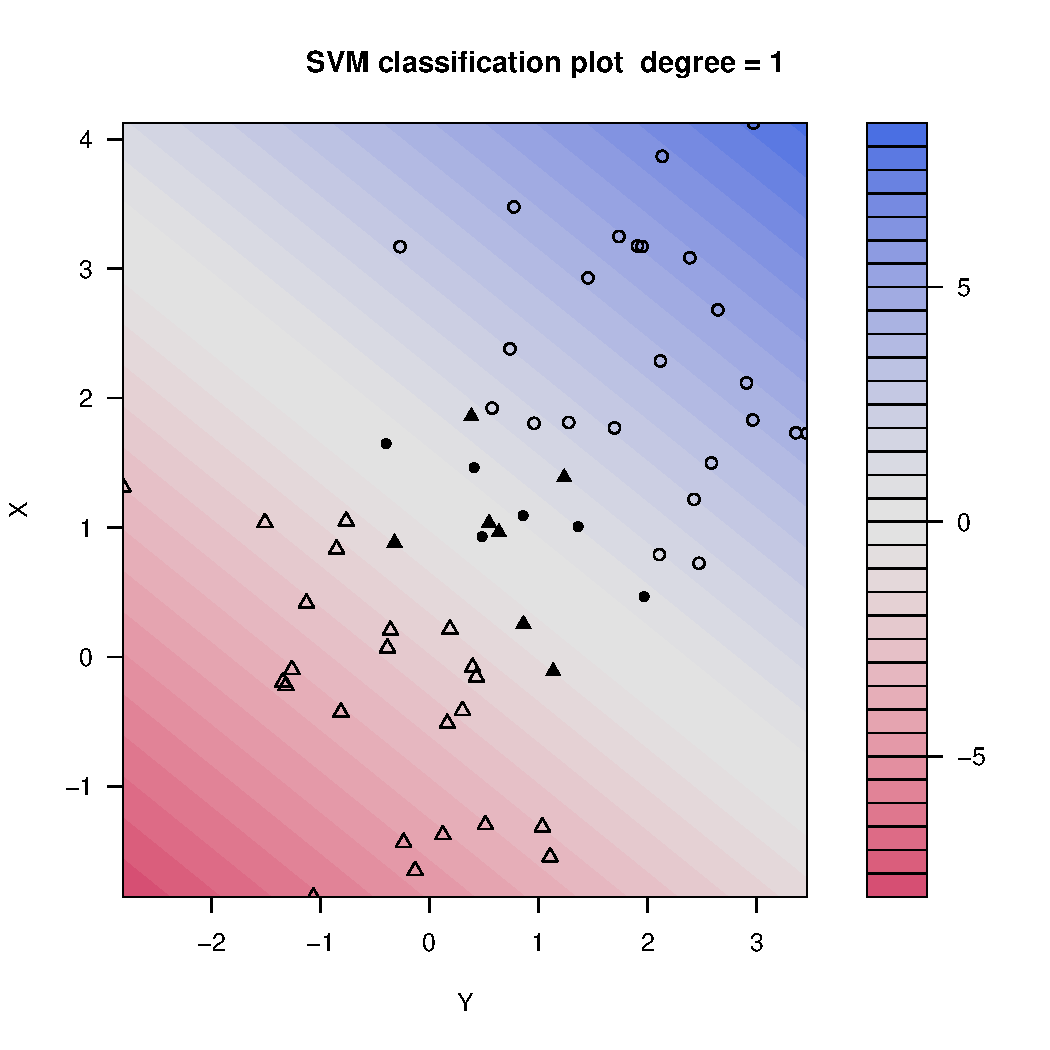
\includegraphics[width=4cm]{Graphics/Problema_01/Experiment_02_1.pdf}
		\caption{}
	\end{subfigure}
	\begin{subfigure}{4cm}
		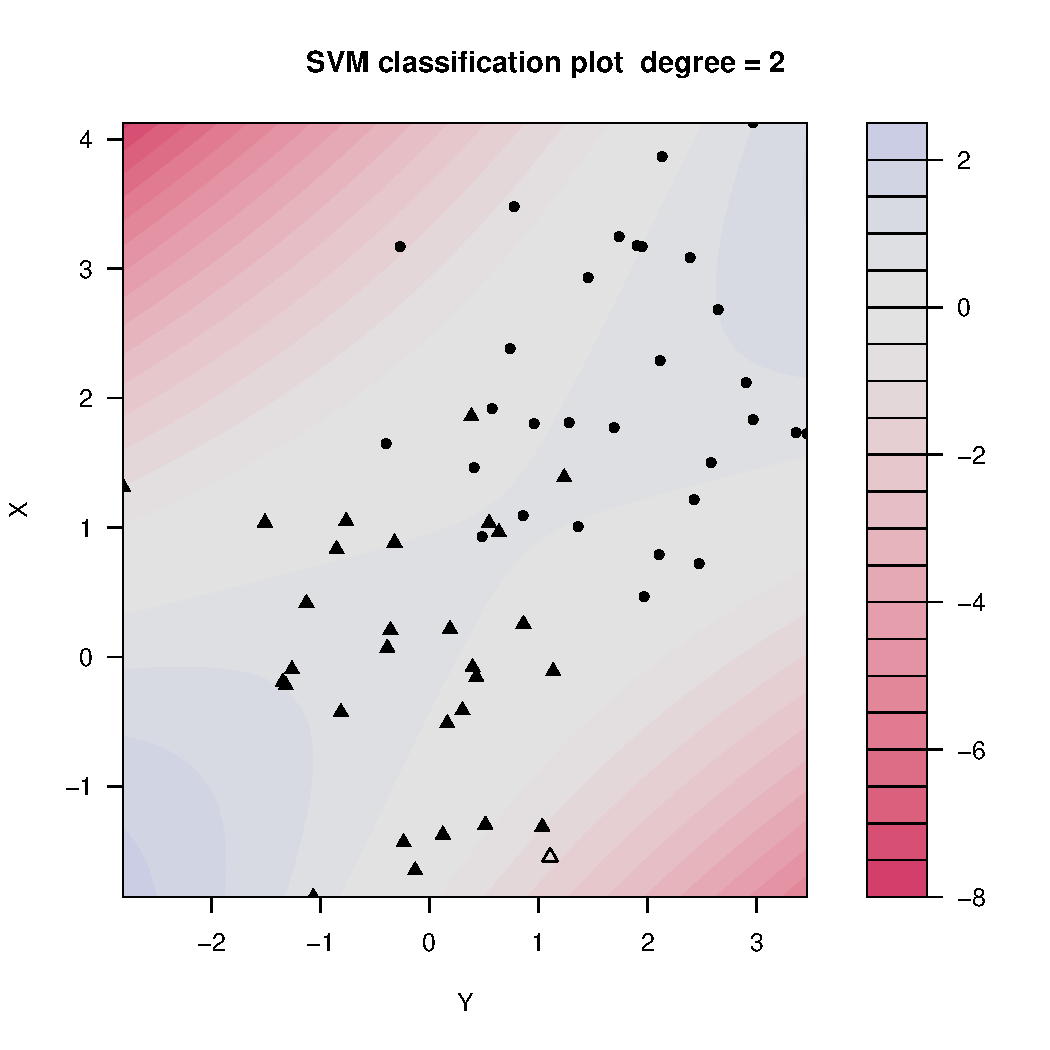
\includegraphics[width=4cm]{Graphics/Problema_01/Experiment_02_2.pdf}
		\caption{}
	\end{subfigure}
	\begin{subfigure}{4cm}
		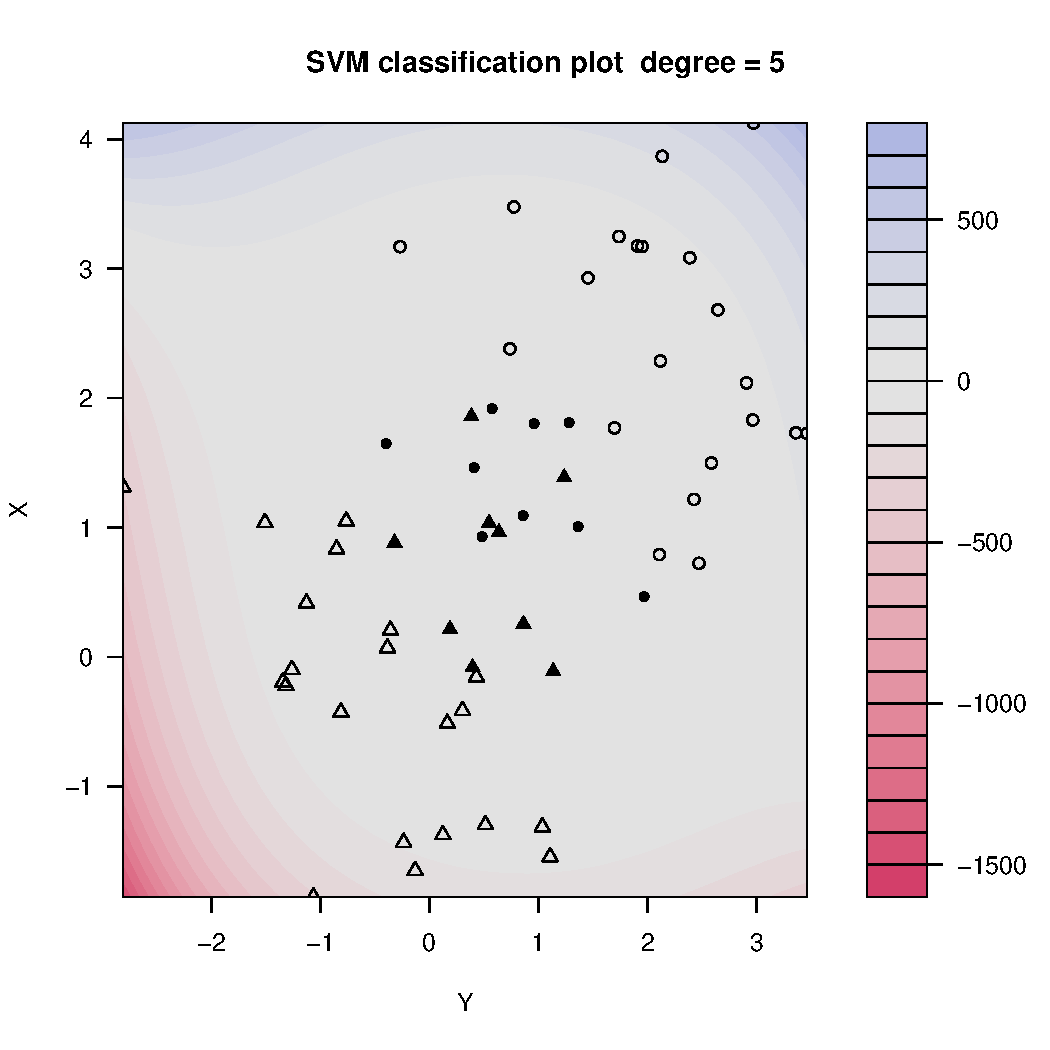
\includegraphics[width=4cm]{Graphics/Problema_01/Experiment_02_3.pdf}
		\caption{}
	\end{subfigure}
	\begin{subfigure}{4cm}
		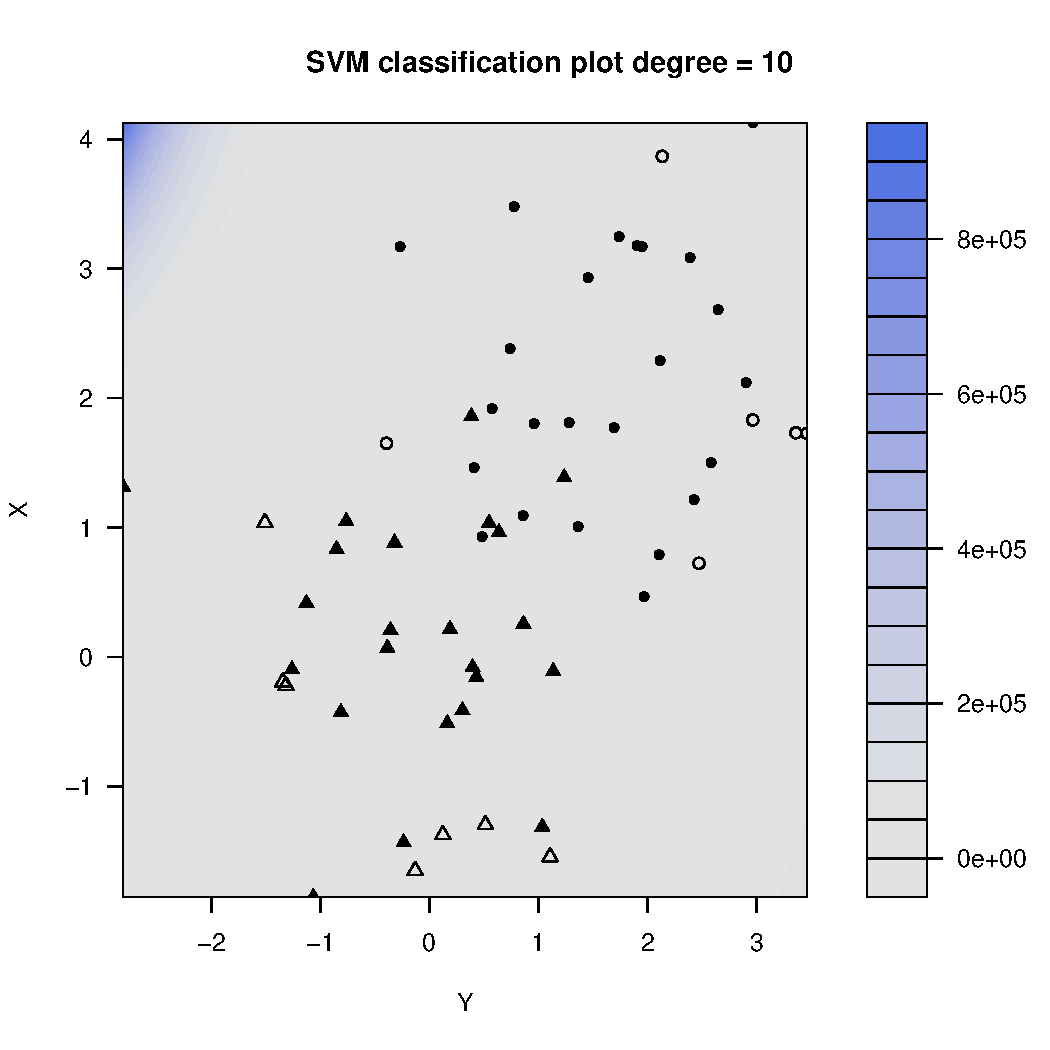
\includegraphics[width=4cm]{Graphics/Problema_01/Experiment_02_4.pdf}
		\caption{}
	\end{subfigure}
	\caption{}
\end{figure}

\subsection*{Experimento 3}

\textbf{¿Cuál es el efecto de cambiar el parámetro de kernel de base radial?}

\begin{figure}[H]
	\centering
	\begin{subfigure}{4cm}
		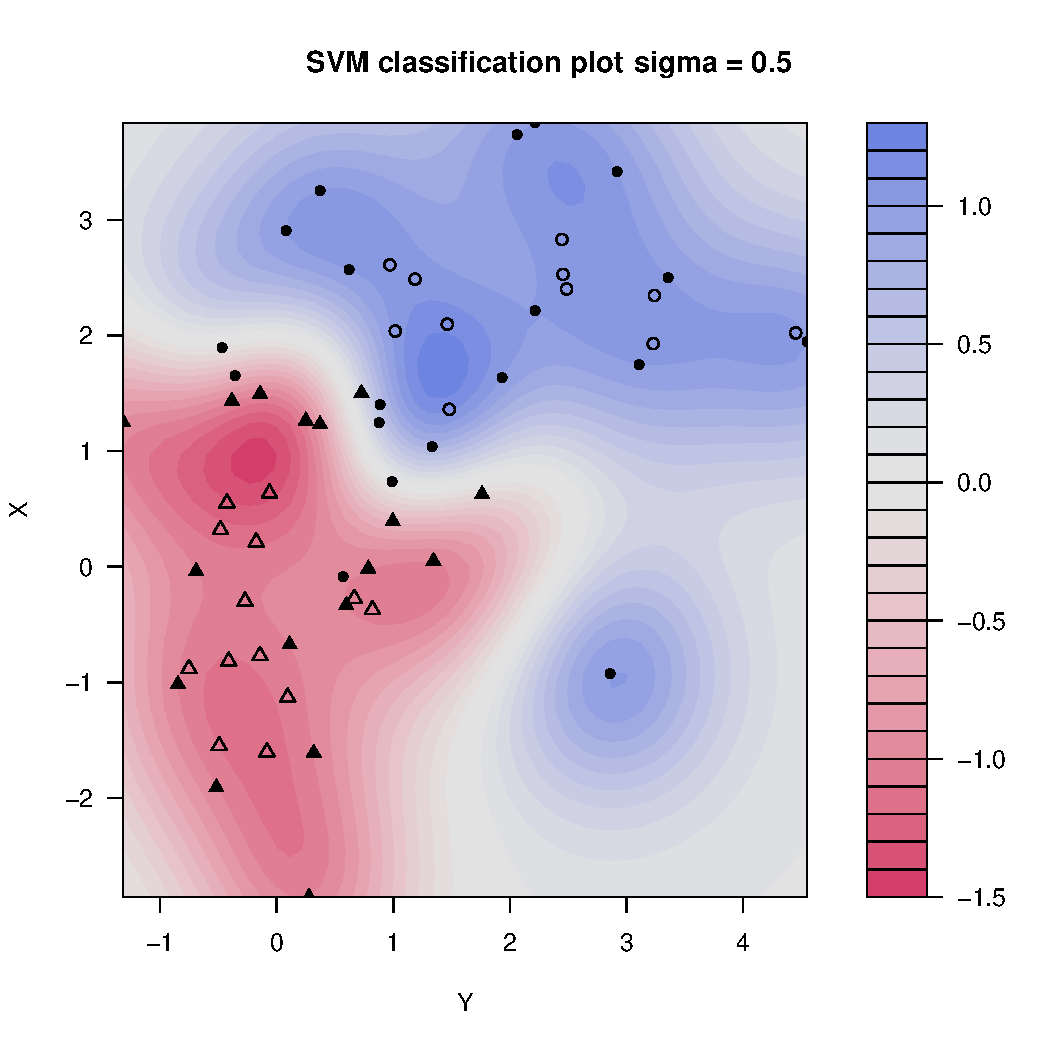
\includegraphics[width=4cm]{Graphics/Problema_01/Experiment_03_1.pdf}
		\caption{}
	\end{subfigure}
	\begin{subfigure}{4cm}
		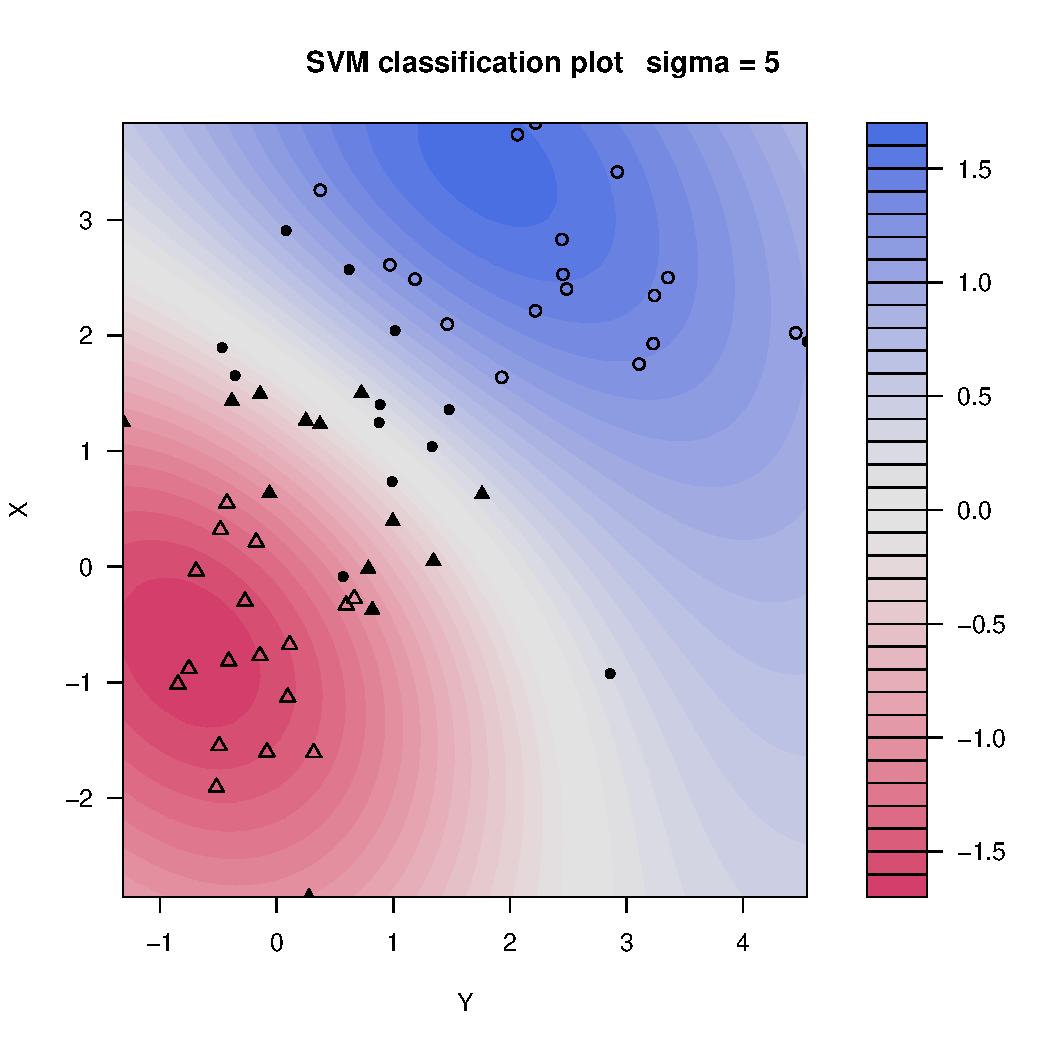
\includegraphics[width=4cm]{Graphics/Problema_01/Experiment_03_2.pdf}
		\caption{}
	\end{subfigure}
	\begin{subfigure}{4cm}
		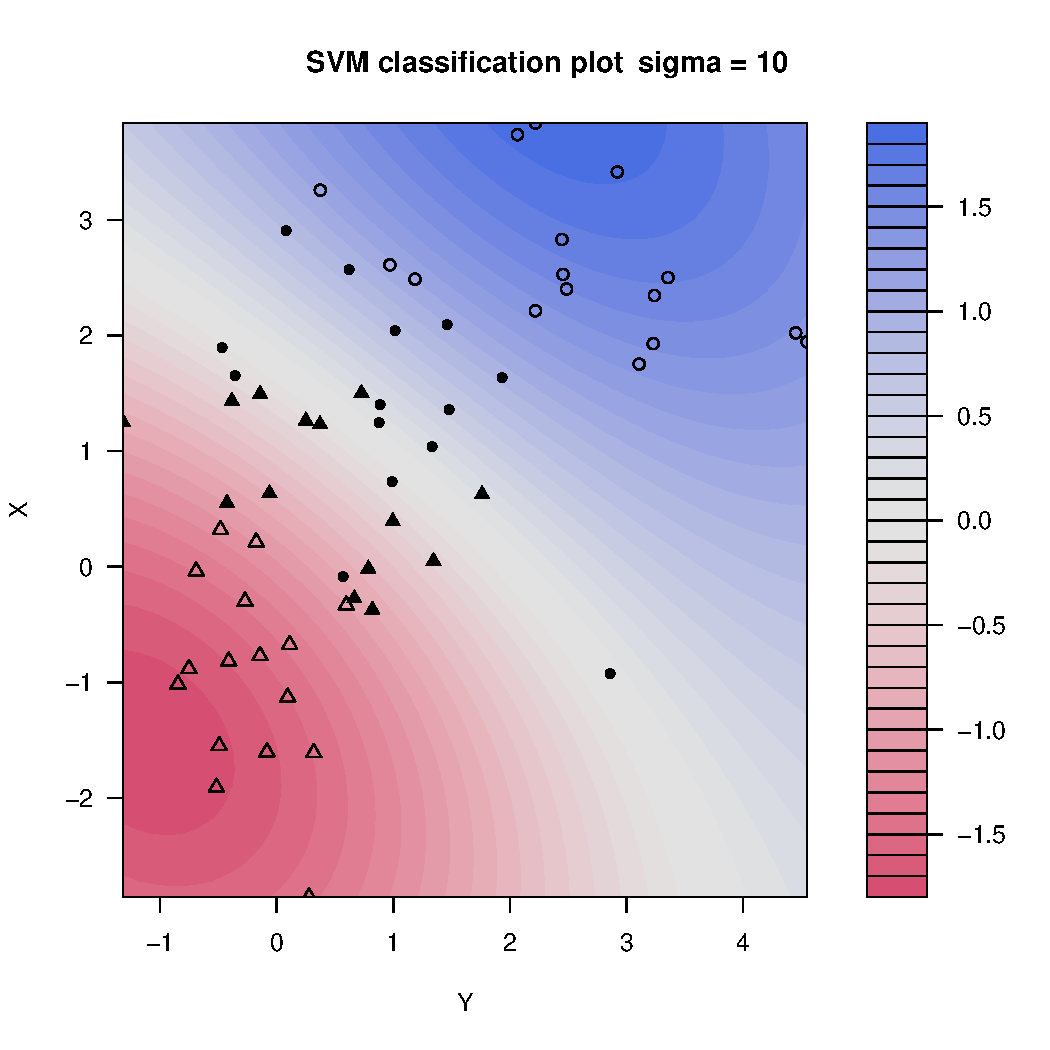
\includegraphics[width=4cm]{Graphics/Problema_01/Experiment_03_3.pdf}
		\caption{}
	\end{subfigure}
	\begin{subfigure}{4cm}
		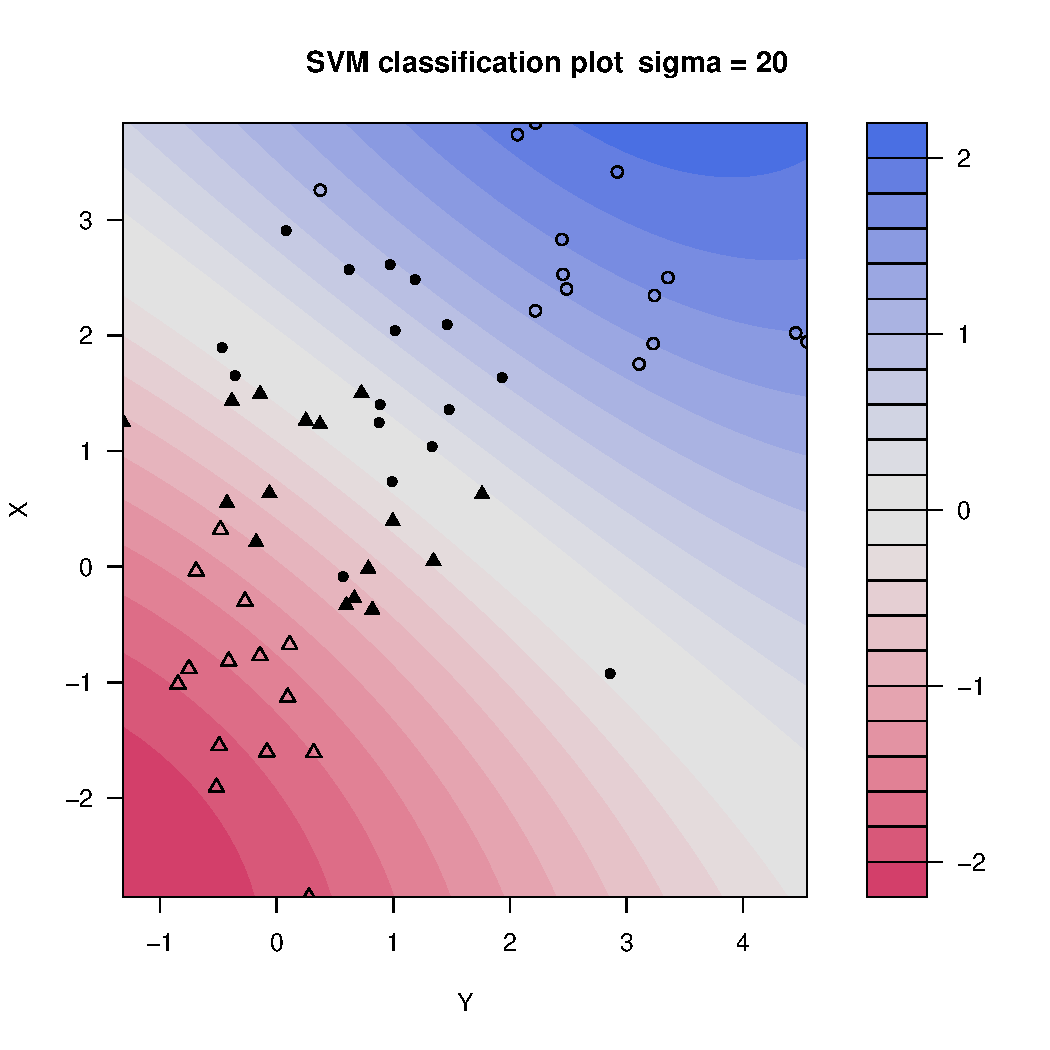
\includegraphics[width=4cm]{Graphics/Problema_01/Experiment_03_4.pdf}
		\caption{}
	\end{subfigure}
	\caption{}
\end{figure}

\subsection*{Experimento 4}

\textbf{¿Cuál es el efecto de cambiar el parámetro $\sigma$ del kernel de base radial?}

\begin{figure}[H]
	\centering
	\begin{subfigure}{4cm}
		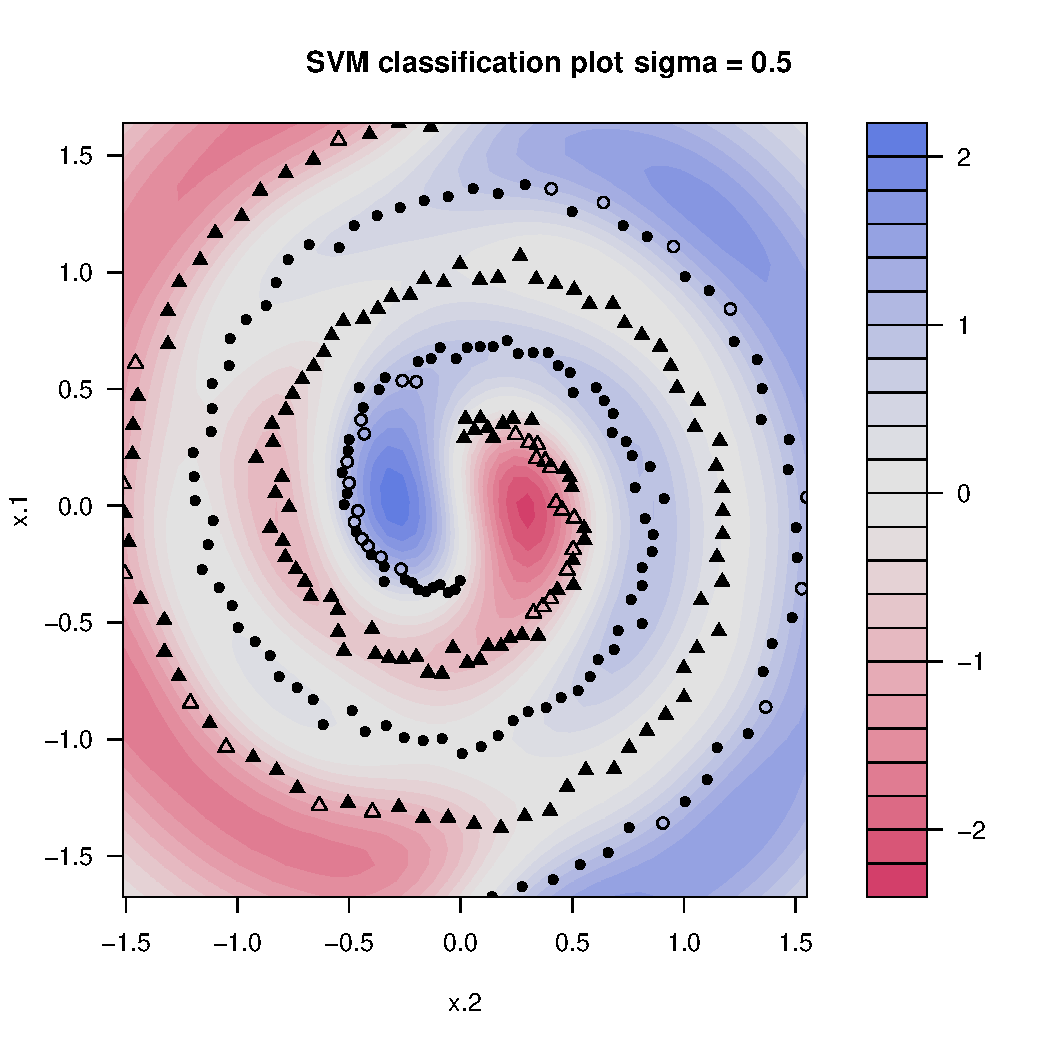
\includegraphics[width=4cm]{Graphics/Problema_01/Experiment_04_1.pdf}
		\caption{}
	\end{subfigure}
	\begin{subfigure}{4cm}
		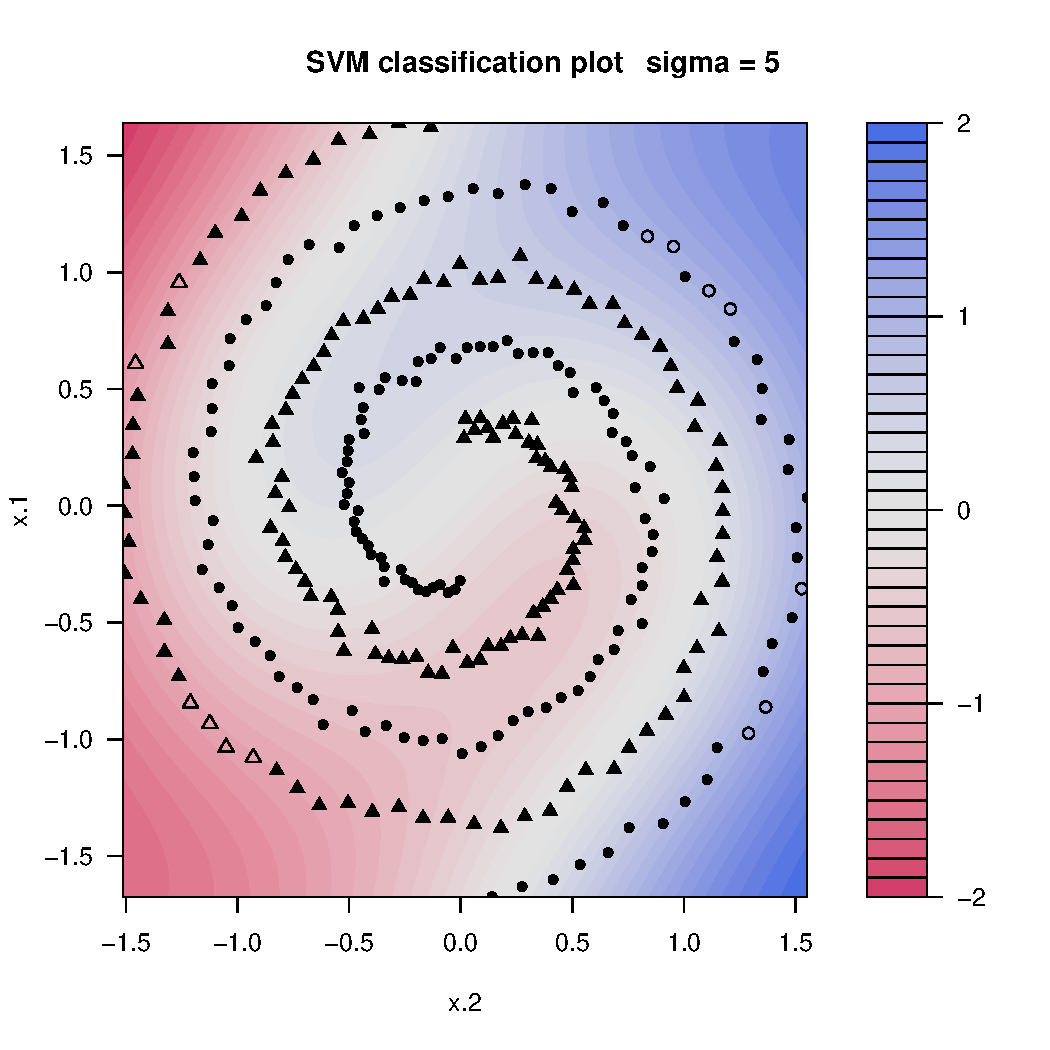
\includegraphics[width=4cm]{Graphics/Problema_01/Experiment_04_2.pdf}
		\caption{}
	\end{subfigure}
	\begin{subfigure}{4cm}
		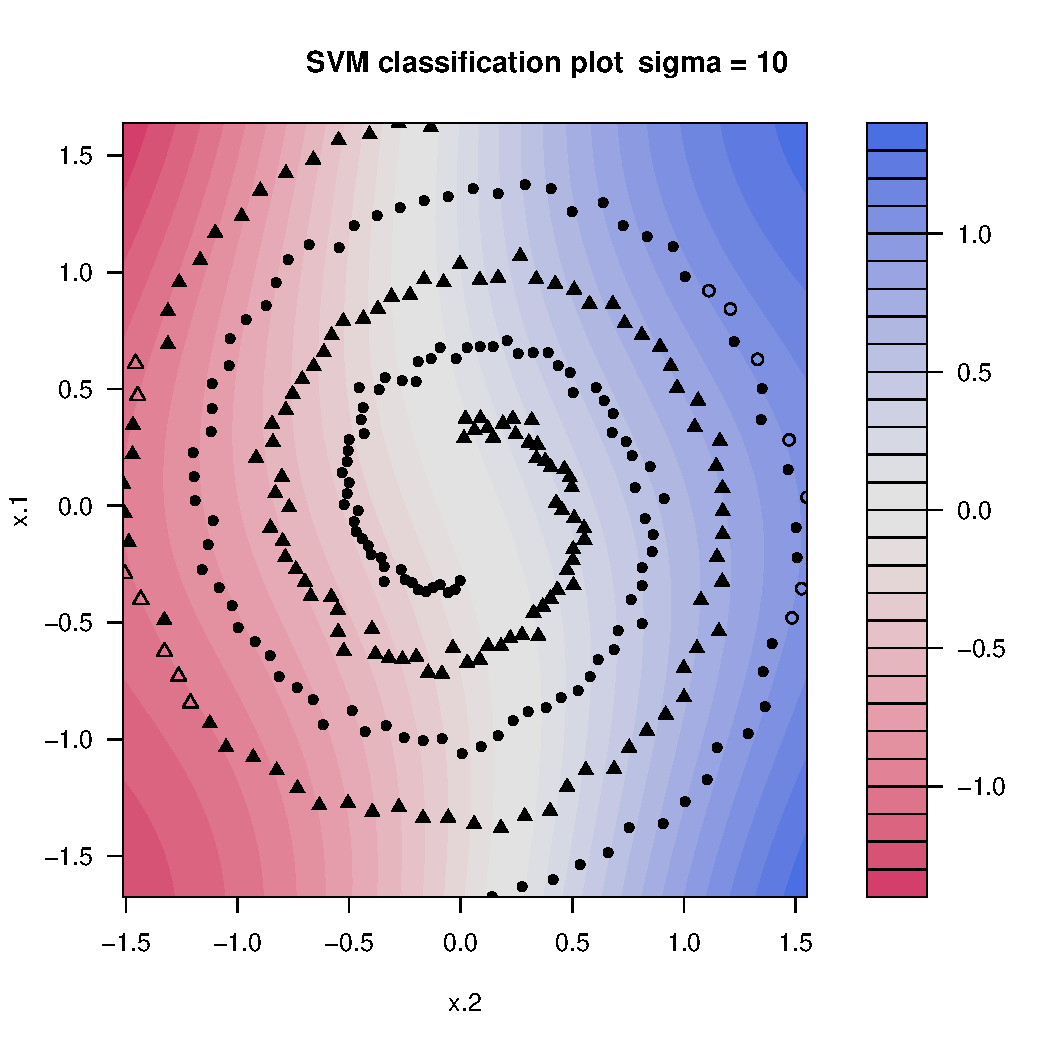
\includegraphics[width=4cm]{Graphics/Problema_01/Experiment_04_3.pdf}
		\caption{}
	\end{subfigure}
	\begin{subfigure}{4cm}
		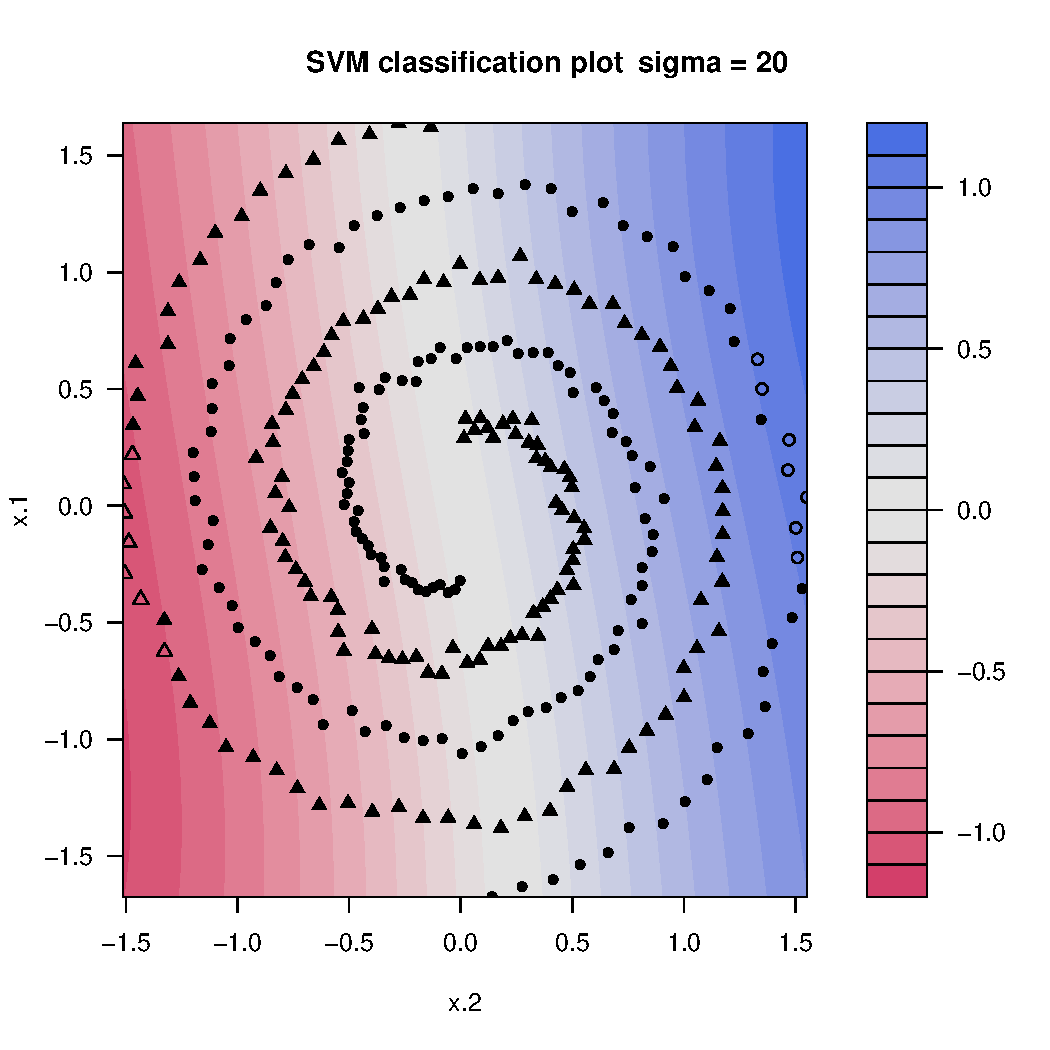
\includegraphics[width=4cm]{Graphics/Problema_01/Experiment_04_4.pdf}
		\caption{}
	\end{subfigure}
	\caption{}
\end{figure}